\documentclass[aspectratio=169,11pt]{beamer}

\usetheme{Madrid}
\usefonttheme{professionalfonts}
\usepackage[T1]{fontenc}
\usepackage{lmodern}
\usepackage{tikz}
\usetikzlibrary{arrows.meta,backgrounds,calc,fit,positioning}

\definecolor{HundoInk}{HTML}{172033}
\definecolor{HundoBlue}{HTML}{2F5E8F}
\definecolor{HundoTeal}{HTML}{1B8A8F}
\definecolor{HundoGold}{HTML}{C08A1E}
\definecolor{HundoRed}{HTML}{B64848}
\definecolor{HundoSoft}{HTML}{F4F7FB}
\definecolor{HundoLine}{HTML}{9AA7B8}

\setbeamercolor{normal text}{fg=HundoInk,bg=white}
\setbeamercolor{structure}{fg=HundoBlue}
\setbeamercolor{frametitle}{fg=white,bg=HundoBlue}
\setbeamercolor{title}{fg=white,bg=HundoBlue}
\setbeamercolor{subtitle}{fg=white}
\setbeamercolor{block title}{fg=white,bg=HundoBlue}
\setbeamercolor{block body}{fg=HundoInk,bg=HundoSoft}
\setbeamercolor{alerted text}{fg=HundoRed}

\setbeamertemplate{navigation symbols}{}
\setbeamertemplate{itemize item}{\color{HundoTeal}\small$\blacktriangleright$}
\setbeamertemplate{itemize subitem}{\color{HundoGold}\scriptsize$\bullet$}
\setbeamertemplate{footline}{
  \leavevmode
  \begin{beamercolorbox}[wd=\paperwidth,ht=2.6ex,dp=1.1ex,leftskip=1.2em,rightskip=1.2em plus 1fil]{author in head/foot}
    \color{HundoInk!70}FM Team Hundo\hfill\insertframenumber/\inserttotalframenumber
  \end{beamercolorbox}
}

\title[FM Team Hundo]{FM Team Hundo}
\subtitle{How the project turns Forbidden Memories progress into a live team race}
\author{}
\date{}

\newcommand{\statcard}[3]{%
  \begin{block}{#1}
    {\large\textbf{#2}}\par
    \vspace{0.25em}
    #3
  \end{block}
}
\newcommand{\flowbadge}[1]{%
  \tikz[baseline=-0.55ex]\node[
    circle,
    draw=HundoInk!55,
    fill=white,
    minimum size=12pt,
    inner sep=1pt,
    font=\bfseries\tiny
  ]{#1};
}

\begin{document}

\begin{frame}[plain]
  \begin{tikzpicture}[remember picture,overlay]
    \fill[HundoBlue] (current page.south west) rectangle (current page.north east);
    \fill[HundoTeal!80] (current page.south west) rectangle ($(current page.south east)+(0,1.15)$);
    \fill[HundoGold] ($(current page.south west)+(0,1.15)$) rectangle ($(current page.south west)+(2.4,1.32)$);
  \end{tikzpicture}
  \vspace{1.25cm}
  {\color{white}\Huge\bfseries FM Team Hundo\par}
  \vspace{0.35cm}
  {\color{white}\Large A live, team-based Yu-Gi-Oh! Forbidden Memories collection race\par}
  \vspace{1.0cm}
  {\color{white}\large One shared goal: complete the team's card library while the software proves, tracks, and broadcasts the progress.}
\end{frame}

\begin{frame}{The Event Experience}
  \begin{columns}[T,onlytextwidth]
    \begin{column}{0.32\textwidth}
      \statcard{Players}{Play normally}{The emulator detects important moments: drops, fusions, rituals, and starchip totals.}
    \end{column}
    \begin{column}{0.32\textwidth}
      \statcard{Teams}{Build one library}{Every valid acquisition updates a shared team library and a race toward 100 percent completion.}
    \end{column}
    \begin{column}{0.32\textwidth}
      \statcard{Viewers}{Watch it unfold}{Dashboards, overlays, and commentary tools turn quiet game events into broadcast moments.}
    \end{column}
  \end{columns}

  \vspace{0.45cm}
  \begin{center}
    \Large\textbf{The project is the connective tissue between local gameplay, official scoring, and a watchable live show.}
  \end{center}
\end{frame}

\begin{frame}{Player Setup: Trust Before Tracking}
  \begin{columns}[T,onlytextwidth]
    \begin{column}{0.48\textwidth}
      \begin{block}{What players do}
        \begin{itemize}
          \item Sign in with Twitch on the FM Team Hundo website.
          \item Join or receive a team assignment.
          \item Download a credentials file for FM\_Sentinel.
          \item Stream gameplay from the registered Twitch account or alt account.
        \end{itemize}
      \end{block}
    \end{column}
    \begin{column}{0.48\textwidth}
      \begin{block}{Why it matters}
        \begin{itemize}
          \item Twitch identity ties game updates to a real participant.
          \item Credentials let the local tool post only for that player.
          \item Team assignment decides which library receives progress.
          \item Streaming keeps the run reviewable and restream-ready.
        \end{itemize}
      \end{block}
    \end{column}
  \end{columns}
\end{frame}

\begin{frame}{Game Events Leave the Emulator}
  \centering
  \resizebox{0.96\textwidth}{!}{%
  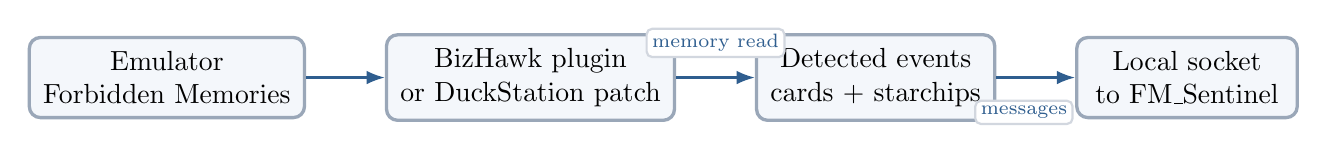
\begin{tikzpicture}[
    node distance=1.0cm,
    eventbox/.style={draw=HundoLine, fill=HundoSoft, rounded corners=4pt, very thick, align=center, minimum width=2.8cm, minimum height=1.0cm, inner sep=5pt},
    flow/.style={-Latex, thick, color=HundoBlue},
    arrowlabel/.style={fill=white, draw=HundoLine!45, rounded corners=2pt, inner sep=2pt, align=center, font=\scriptsize}
  ]
    \node[eventbox] (emu) {Emulator\\Forbidden Memories};
    \node[eventbox,right=of emu] (watcher) {BizHawk plugin\\or DuckStation patch};
    \node[eventbox,right=of watcher] (events) {Detected events\\cards + starchips};
    \node[eventbox,right=of events] (local) {Local socket\\to FM\_Sentinel};

    \draw[flow] (emu) -- (watcher);
    \draw[flow] (watcher) -- node[arrowlabel,above=7pt]{memory read} (events);
    \draw[flow] (events) -- node[arrowlabel,below=8pt,pos=.35]{messages} (local);
  \end{tikzpicture}
  }

  \vspace{0.65cm}
  \begin{block}{Plain-language version}
    The emulator integration watches the game for moments that count. When a player wins a drop, creates a fusion, performs a ritual, or changes starchips, it sends a small event to the local bridge. Most progress does not need manual reporting.
  \end{block}
\end{frame}

\begin{frame}{FM\_Sentinel: The Local Bridge}
  \begin{columns}[T,onlytextwidth]
    \begin{column}{0.48\textwidth}
      \begin{block}{On the player machine}
        \begin{itemize}
          \item Opens a local connection for the emulator.
          \item Reads the player's downloaded credentials file.
          \item Checks that the website accepts those credentials.
          \item Verifies compatible event protocol versions when release builds are stamped.
        \end{itemize}
      \end{block}
    \end{column}
    \begin{column}{0.48\textwidth}
      \begin{block}{Toward the server}
        \begin{itemize}
          \item Batches emulator events.
          \item Posts them to the collection API.
          \item Retries when the server connection fails.
          \item Prints human-readable feedback for the player.
        \end{itemize}
      \end{block}
    \end{column}
  \end{columns}

  \vspace{0.35cm}
  \begin{center}
    \large\textbf{FM\_Sentinel keeps emulator-specific code away from the public website and gives players one simple local tool.}
  \end{center}
\end{frame}

\begin{frame}{The Server: Official Source of Truth}
  \small
  \begin{columns}[T,onlytextwidth]
    \begin{column}{0.5\textwidth}
      \begin{block}{Website and accounts}
        \begin{itemize}
          \item Twitch login creates or updates player profiles.
          \item Players can download fresh credentials and set an alt stream account.
          \item Admin tools create teams and assign unassigned users.
        \end{itemize}
      \end{block}
      \begin{block}{Collection API}
        \begin{itemize}
          \item Validates API keys.
          \item Rejects impossible card IDs and unobtainable cards.
          \item Saves every accepted player update with a server timestamp.
        \end{itemize}
      \end{block}
    \end{column}
    \begin{column}{0.46\textwidth}
      \begin{block}{Live game state}
        \begin{itemize}
          \item Rebuilds each team's library from stored updates.
          \item Calculates unbuyables, buyable cost, BEWD and Gate Guardian exceptions, and completion.
          \item Broadcasts player and team updates over firehose WebSockets.
          \item Can resolve acquisition moments to Twitch VOD links when enabled.
        \end{itemize}
      \end{block}
    \end{column}
  \end{columns}
\end{frame}

\begin{frame}{How the Parts Work Together}
  \centering
  \resizebox{\textwidth}{!}{%
  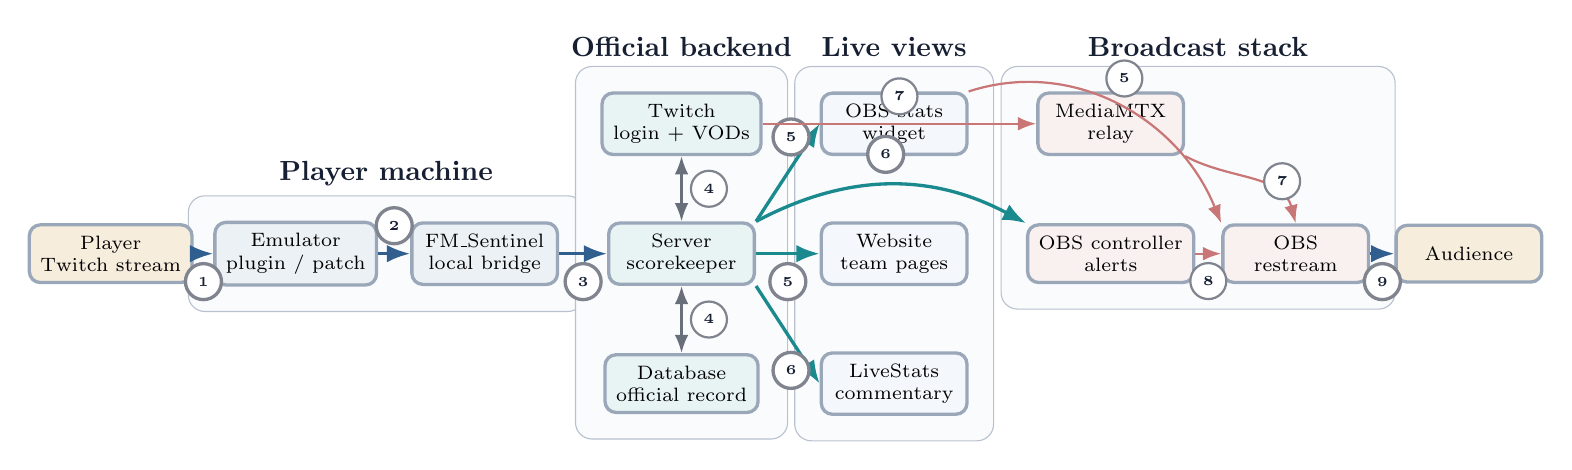
\begin{tikzpicture}[
    font=\scriptsize,
    x=1cm,
    y=1cm,
    box/.style={draw=HundoLine, rounded corners=4pt, very thick, fill=white, align=center, minimum width=1.85cm, minimum height=0.72cm, inner sep=4pt},
    actor/.style={box, fill=HundoGold!15},
    local/.style={box, fill=HundoBlue!9},
    server/.style={box, fill=HundoTeal!10},
    surface/.style={box, fill=HundoSoft},
    broadcast/.style={box, fill=HundoRed!8},
    group/.style={draw=HundoLine!70, rounded corners=6pt, fill=HundoSoft!45, inner sep=9pt},
    flow/.style={-Latex, very thick, color=HundoBlue},
    live/.style={-Latex, very thick, color=HundoTeal},
    control/.style={-Latex, thick, color=HundoRed!75},
    data/.style={Latex-Latex, thick, color=HundoInk!65},
    badge/.style={circle, draw=HundoInk!55, fill=white, minimum size=13pt, inner sep=1pt, font=\bfseries\tiny, text=HundoInk}
  ]
    \node[actor] (player) at (0,2.7) {Player\\Twitch stream};
    \node[local] (emu) at (2.35,2.7) {Emulator\\plugin / patch};
    \node[local] (sentinel) at (4.75,2.7) {FM\_Sentinel\\local bridge};
    \node[server] (api) at (7.25,2.7) {Server\\scorekeeper};
    \node[server] (db) at (7.25,1.05) {Database\\official record};
    \node[server] (twitch) at (7.25,4.35) {Twitch\\login + VODs};

    \node[surface] (web) at (9.95,2.7) {Website\\team pages};
    \node[surface] (widgets) at (9.95,4.35) {OBS stats\\widget};
    \node[surface] (livestats) at (9.95,1.05) {LiveStats\\commentary};

    \node[broadcast] (obsctl) at (12.7,2.7) {OBS controller\\alerts};
    \node[broadcast] (mediamtx) at (12.7,4.35) {MediaMTX\\relay};
    \node[broadcast] (obs) at (15.05,2.7) {OBS\\restream};
    \node[actor] (audience) at (17.25,2.7) {Audience};

    \begin{scope}[on background layer]
      \node[group,fit=(emu)(sentinel),label={[font=\bfseries\color{HundoInk}]above:Player machine}] {};
      \node[group,fit=(api)(db)(twitch),label={[font=\bfseries\color{HundoInk}]above:Official backend}] {};
      \node[group,fit=(web)(widgets)(livestats),label={[font=\bfseries\color{HundoInk}]above:Live views}] {};
      \node[group,fit=(obsctl)(mediamtx)(obs),label={[font=\bfseries\color{HundoInk}]above:Broadcast stack}] {};
    \end{scope}

    \draw[flow] (player) -- node[badge,below=3pt]{1} (emu);
    \draw[flow] (emu) -- node[badge,above=3pt]{2} (sentinel);
    \draw[flow] (sentinel) -- node[badge,below=3pt]{3} (api);
    \draw[data] (api) -- node[badge,right=3pt]{4} (db);
    \draw[data] (api) -- node[badge,right=3pt]{4} (twitch);

    \draw[live] (api) -- node[badge,below=3pt]{5} (web);
    \draw[live] (api.north east) -- node[badge,above=4pt,pos=.55]{5} (widgets.west);
    \draw[live] (api.south east) -- node[badge,below=4pt,pos=.55]{6} (livestats.west);
    \draw[live] (api.north east) to[out=28,in=152] node[badge,above=4pt,pos=.48]{6} (obsctl.north west);

    \draw[control] (twitch.east) -- node[badge,above=3pt]{7} (mediamtx.west);
    \draw[control] (mediamtx.south east) to[out=-28,in=105] node[badge,right=3pt,pos=.52]{7} (obs.north);
    \draw[control] (obsctl) -- node[badge,below=3pt]{8} (obs);
    \draw[control] (widgets.north east) to[out=18,in=112] node[badge,above=4pt,pos=.52]{5} (obs.north west);
    \draw[flow] (obs) -- node[badge,below=3pt]{9} (audience);
  \end{tikzpicture}
  }
  \vspace{0.25cm}

  {\scriptsize
  \begin{tabular}{@{}ll@{\hspace{0.55cm}}ll@{\hspace{0.55cm}}ll@{}}
    \flowbadge{1} & player plays/streams &
    \flowbadge{2} & emulator detects events &
    \flowbadge{3} & FM\_Sentinel posts updates \\
    \flowbadge{4} & backend stores/checks &
    \flowbadge{5} & pages/widgets publish state &
    \flowbadge{6} & firehose feeds live tools \\
    \flowbadge{7} & live video is relayed &
    \flowbadge{8} & OBS scenes are controlled &
    \flowbadge{9} & audience sees the show
  \end{tabular}
  }
\end{frame}

\begin{frame}{Live Views and Broadcast Automation}
  \begin{columns}[T,onlytextwidth]
    \begin{column}{0.48\textwidth}
      \begin{block}{For the website and commentary desk}
        \begin{itemize}
          \item Home page compares team progress.
          \item Team pages show library grids, latest cards, members, and completion banners.
          \item Player pages show each person's recent non-starchip activity.
          \item LiveStats gives commentary a compact, always-updating operations view.
        \end{itemize}
      \end{block}
    \end{column}
    \begin{column}{0.48\textwidth}
      \begin{block}{For the restream}
        \begin{itemize}
          \item Streamlink and FFmpeg can forward Twitch streams into MediaMTX.
          \item The OBS controller discovers stream paths and builds managed scenes.
          \item A team firehose event can trigger a scene cut, banner, intro, and audio focus.
          \item Stats widgets are available as browser sources for OBS layouts.
        \end{itemize}
      \end{block}
    \end{column}
  \end{columns}
\end{frame}

\begin{frame}{Why It Works as a Full Event System}
  \begin{columns}[T,onlytextwidth]
    \begin{column}{0.31\textwidth}
      \begin{block}{One truth}
        Accepted updates are stored centrally, replayed into team libraries, and broadcast to every live surface.
      \end{block}
    \end{column}
    \begin{column}{0.31\textwidth}
      \begin{block}{One release line}
        The server, FM\_Sentinel, and BizHawk plugin share a protocol version in CI release artifacts.
      \end{block}
    \end{column}
    \begin{column}{0.31\textwidth}
      \begin{block}{Many audiences}
        Players get simple setup, organizers get tools, commentators get live state, and viewers get a coherent show.
      \end{block}
    \end{column}
  \end{columns}

  \vspace{0.45cm}
  \begin{center}
    \Large\textbf{FM Team Hundo is a race platform: capture, verify, score, display, and broadcast in one loop.}
  \end{center}
\end{frame}

\end{document}
